\documentclass[11pt,a4paper]{article}
\usepackage[utf8]{inputenc}
\usepackage[T1]{fontenc}
\usepackage[french]{babel}
\usepackage{graphicx}
\usepackage{geometry}
\usepackage{float}
\usepackage{amsmath}
\usepackage{amssymb}
\usepackage{hyperref}
\usepackage{xcolor}
\usepackage[most]{tcolorbox} % Pour les beaux encadrés mathématiques
\usepackage{setspace} % Pour aérer le texte

% Paramètres de mise en page pour aérer le document
\geometry{top=2.5cm, bottom=2.5cm, left=2.5cm, right=2.5cm}
\setlength{\parskip}{0.8em} % Espacement entre les paragraphes
\setstretch{1.10} % Interligne légèrement augmenté

% Définition des couleurs pour les encadrés
\definecolor{thmblue}{RGB}{230, 240, 255}
\definecolor{borderblue}{RGB}{0, 80, 160}
\definecolor{defgray}{RGB}{245, 245, 245}
\definecolor{bordergray}{RGB}{100, 100, 100}

\title{\textbf{\Huge Rapport de Projet} \\ \vspace{0.5cm} \Large Modélisation Spatiale des Extrêmes de Mortalité COVID-19 aux États-Unis (EVT-CART)}
\author{Équipe de Projet}
\date{\today}

\begin{document}

\begin{center}

{\Large École Nationale des Ponts et Chaussées}

\vspace{2cm}

% Logo

\includegraphics[width=0.35\textwidth]{logo_ponts.jpg}

\vspace{2cm}

{\Large \textbf{Projet de département IMI}}\\
\vspace{0.3cm}
{\itshape Rapport}

\vspace{1.5cm}

\hrule
\vspace{0.4cm}
{\Large \textbf{Modélisation Spatiale des Extrêmes de Mortalité COVID-19 aux États-Unis (EVT-CART)}}
\vspace{0.4cm}
\hrule

\vspace{2cm}

{\large \textbf{Membres du groupe :}}

\vspace{0.5cm}

\begin{center}
Eliott Delhaye\\
Chloé Spittael\\
Camille Viénot\\
Paul-Emile Marcus
\end{center}

\vfill

{\large 2025 / 2026}

\end{center}

\newpage



\begin{abstract}
\noindent L'évaluation du risque pandémique ne peut se limiter à l'étude des moyennes ; elle nécessite d'anticiper les scénarios catastrophes. Ce projet s'attache à modéliser les taux de mortalité extrêmes liés à la COVID-19 à l'échelle des comtés américains. En nous appuyant sur les fondements mathématiques de la Théorie des Valeurs Extrêmes (TVE) couplés aux arbres de régression (EVT-CART) et à l'interpolation géostatistique (Krigeage), nous proposons une cartographie territorialisée du risque extrême. Ce rapport détaille le socle théorique de cette modélisation, l'analyse des résultats obtenus par notre équipe, ainsi que les limites inhérentes à l'estimation des queues de distribution sur de petits échantillons spatiaux.
\end{abstract}

\tableofcontents
\newpage

\section{Introduction}

\subsection{Contexte et Problématique}
L'analyse classique des données épidémiologiques repose majoritairement sur des modélisations de la tendance centrale (moyenne, médiane). Or, face à un choc systémique tel qu'une pandémie, le véritable enjeu pour les décideurs publics et les assureurs réside dans l'anticipation des scénarios du pire : les extrêmes de surmortalité. 

La difficulté majeure réside dans l'hétérogénéité du territoire américain. La question centrale de notre étude est donc la suivante : \textbf{Comment modéliser et cartographier rigoureusement les queues de distribution de la mortalité COVID-19 en tenant compte des disparités démographiques, géographiques et socio-économiques locales ?}

\subsection{État de l'art et cadre du projet}
Pour répondre à ce défi, nous nous appuyons sur la \textbf{Théorie des Valeurs Extrêmes (TVE)}. Historiquement utilisée en hydrologie ou en finance, la TVE permet de modéliser la probabilité d'occurrence d'événements plus extrêmes que ceux déjà observés (inférence en dehors du support de l'échantillon historique).

Cependant, l'application classique de la TVE suppose des données indépendantes et identiquement distribuées (i.i.d.), une hypothèse intenable à l'échelle d'un pays entier. Pour capturer l'hétérogénéité spatiale, nous avons implémenté l'algorithme \textbf{EVT-CART} (Generalized Pareto Regression Trees), récemment développé par Farkas, Thomas et al. (2021).

\section{Fondements Mathématiques de la Théorie des Valeurs Extrêmes}

\subsection{Limites de la statistique classique et principe de la TVE}
Les méthodes statistiques traditionnelles (Théorème Central Limite, lois normales) sont conçues pour décrire le cœur d'une distribution. Appliquées aux queues de distribution (les événements rares), elles sous-estiment drastiquement la probabilité d'occurrence des valeurs extrêmes. 

Il existe deux grandes approches en TVE : l'étude des maxima par blocs (théorème de Fisher-Tippett et loi GEV) et l'étude des dépassements de seuil. Dans ce projet, nous utilisons l'approche \textbf{Peaks over Threshold (PoT)}, plus efficiente en termes d'utilisation des données.

Soit $Y_1, \dots, Y_n$ des variables aléatoires i.i.d. de fonction de répartition inconnue $F$. Nous nous intéressons au comportement des excès $Y - u$, conditionnellement au fait que la variable dépasse un seuil élevé $u$.

\subsection{Le Théorème fondamental de l'approche PoT}

\begin{tcolorbox}[colback=thmblue, colframe=borderblue, title=\textbf{Théorème de Pickands-Balkema-de Haan (1974)}, rounded corners]
Ce théorème stipule que, pour une large classe de distributions sous-jacentes $F$, et pour un seuil $u$ suffisamment grand, la loi des excès tend asymptotiquement vers une \textbf{loi de Pareto Généralisée (GPD)} :
\begin{equation}
    \mathbb{P}(Y - u > y \mid Y > u) \approx 1 - G_{\xi, \sigma}(y) = \left( 1 + \frac{\xi y}{\sigma} \right)^{-1/\xi}
\end{equation}
\textit{Définie sur l'ensemble $\{y : y > 0 \text{ et } (1 + \xi y / \sigma) > 0\}$.}
\end{tcolorbox}

Dans cette formulation :
\begin{itemize}
    \item \textbf{$\sigma > 0$} est le paramètre d'échelle (qui dépend du seuil $u$), mesurant la dispersion des extrêmes.
    \item \textbf{$\xi \in \mathbb{R}$} est le paramètre de forme (souvent noté $\xi$ dans la littérature), qui caractérise le comportement de la queue de distribution.
\end{itemize}

\subsection{Interprétation épidémiologique du paramètre de forme ($\xi$)}

Le paramètre $\xi$ définit trois domaines d'attraction pour les extrêmes, dont l'interprétation est vitale pour notre projet :

\begin{tcolorbox}[colback=defgray, colframe=bordergray, title=\textbf{Les trois domaines d'attraction}, arc=2mm]
\begin{itemize}
    \item \textbf{$\xi > 0$ (Domaine de Fréchet) :} La distribution présente une queue lourde (décroissance polynomiale). Le risque d'événements cataclysmiques est élevé, modélisant une épidémie "hors de contrôle" sans borne supérieure théorique.
    \item \textbf{$\xi = 0$ (Domaine de Gumbel) :} La queue est légère (décroissance exponentielle).
    \item \textbf{$\xi < 0$ (Domaine de Weibull) :} La distribution possède une \textbf{borne supérieure finie} ($y_{max} = -\sigma / \xi$). Dans notre contexte, cela traduit un "plafond" de surmortalité, reflétant une saturation du taux de mortalité due aux limites démographiques locales.
\end{itemize}
\end{tcolorbox}

\section{Données et Variables de l'Étude}

Notre base de données résulte de la fusion des données de surveillance COVID-19 du CDC et des données socio-démographiques de l'US Census (ACS 2020) à l'échelle des comtés américains.

\subsection{Variables explicatives et ingénierie de la cible}
Au sein de notre équipe de projet, nous avons exploré différentes formulations pour capter la vulnérabilité locale. Outre la densité, l'âge médian, les coordonnées géographiques et le pourcentage de plus de 65 ans, certains d'entre nous ont intégré des variables sociologiques complémentaires (comme l'accès aux soins).

Un travail exploratoire important a été mené sur la \textbf{variable cible ($Y$)} :
\begin{enumerate}
    \item \textit{Décès bruts :} Inefficace car trop trivialement corrélé à la population totale.
    \item \textit{Normalisation par la racine carrée ($Y = \text{décès}/\sqrt{\text{pop}}$) :} Testée avec succès par une partie du groupe pour stabiliser la variance des estimateurs sur les petits comtés.
    \item \textit{Taux d'incidence classique :} Finalement retenue pour ce rapport en raison de son interprétabilité standard.
\end{enumerate}

\begin{tcolorbox}[colback=white, colframe=bordergray]
\textbf{Variable cible finale retenue pour l'analyse :}
$$ Y = \left( \frac{\text{total\_deaths}}{\text{population}} \right) \times 100\,000 $$
\end{tcolorbox}

\begin{figure}[H]
    \centering
    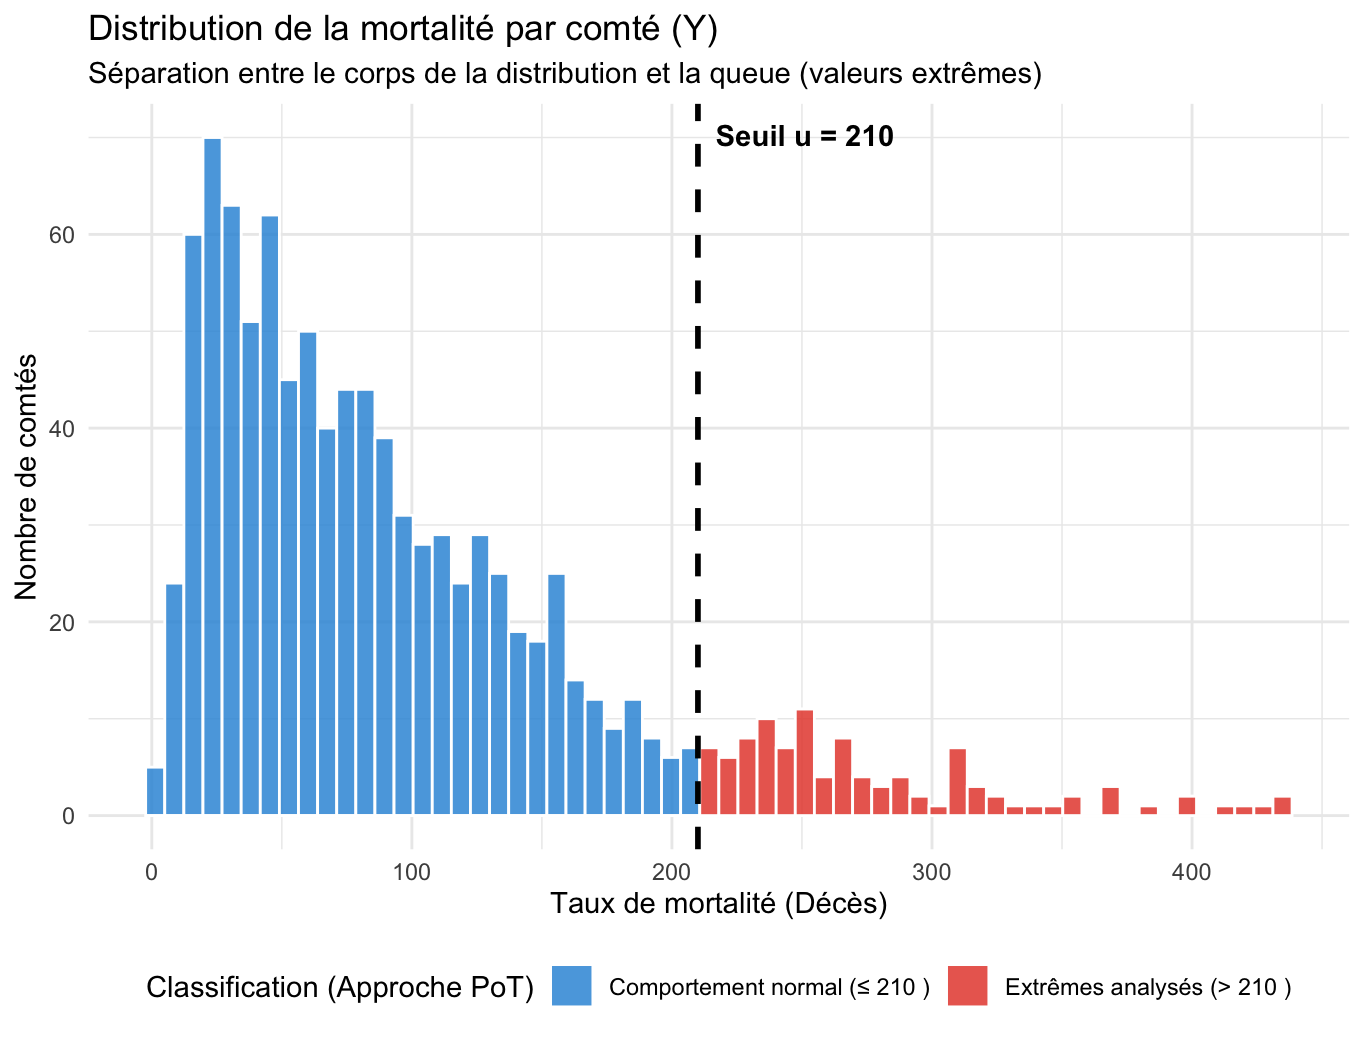
\includegraphics[width=0.7\textwidth]{histogramme1.png}
    \caption{Distribution du taux de mortalité (Y) par comté. La ligne rouge indique le seuil des extrêmes choisi ultérieurement.}
\end{figure}

\section{Modélisation et Analyse des Points Durs}

L'application de la TVE sur des données réelles nécessite de surmonter plusieurs défis méthodologiques, qui constituent la plus-value scientifique de notre démarche.

\subsection{Point dur 1 : Le choix du seuil $u$ (Mean Residual Life)}
Fixer $u$ requiert d'équilibrer le \textbf{biais} (un seuil trop bas viole l'approximation asymptotique) et la \textbf{variance} (un seuil trop haut réduit drastiquement la taille de l'échantillon $n_u$).

Nous avons utilisé le \textit{Mean Residual Life Plot} (MRL). 

\begin{tcolorbox}[colback=thmblue, colframe=borderblue, title=\textbf{Équation de l'Espérance des excès}]
Si la GPD est un modèle valide pour les excès, l'espérance de l'excès moyen au-dessus d'un seuil $u$ doit être une fonction strictement linéaire en $u$ :
\begin{equation}
    E[Y - u \mid Y > u] = \frac{\sigma_u}{1 - \xi} + \frac{\xi u}{1 - \xi}
\end{equation}
\end{tcolorbox}

Sur notre jeu de données (Figure 2), une linéarité nette est observée pour $u \in [210,240]$. Nous avons donc rigoureusement fixé le seuil d'analyse à $u = 210$.

\begin{figure}[H]
    \centering
    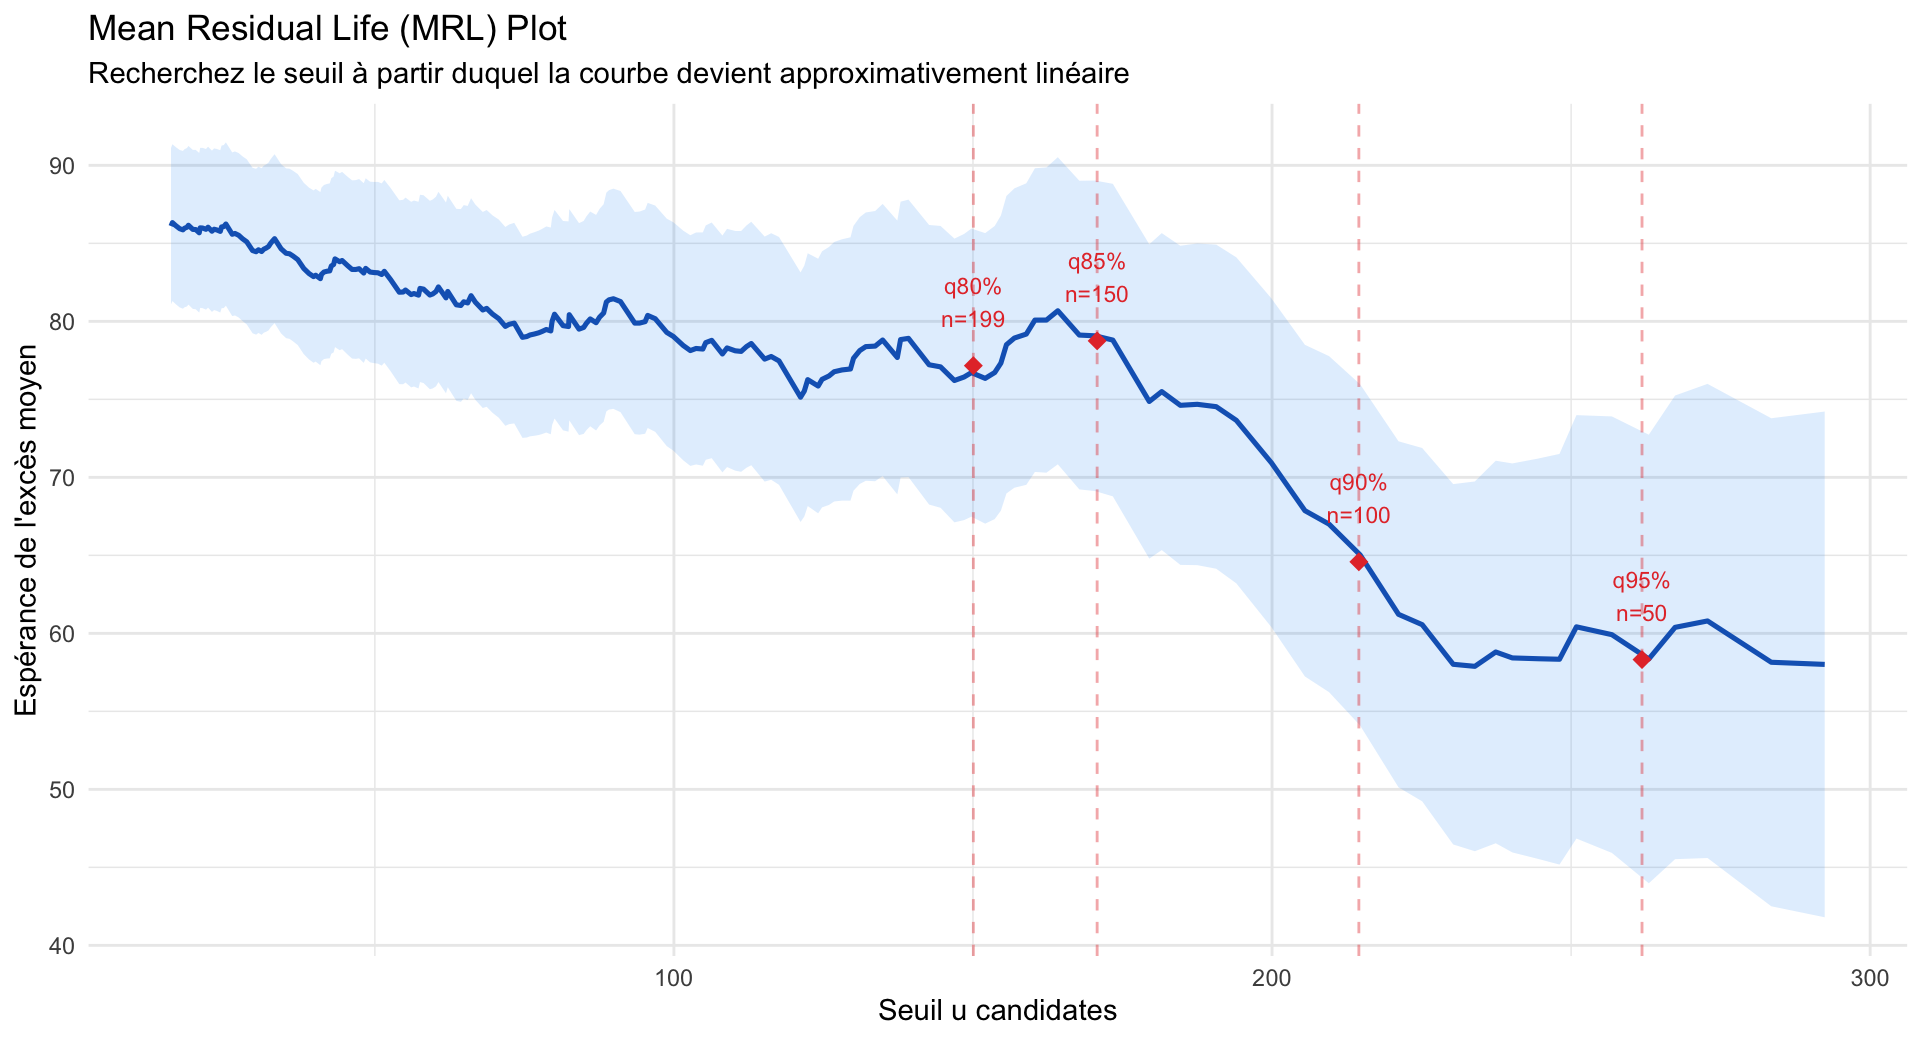
\includegraphics[width=0.7\textwidth]{mrl1.png}
    \caption{Mean Residual Life Plot. La linéarité valide théoriquement l'adéquation d'une GPD au-dessus de 210.}
\end{figure}

\subsection{Point dur 2 : Stabilité des paramètres et justification de l'algorithme CART}

Pour valider le choix du seuil $u$, la littérature (Coles, 2001) recommande de vérifier la propriété fondamentale de \textbf{stabilité par rapport au seuil} de la loi GPD. 

\begin{tcolorbox}[colback=thmblue, colframe=borderblue, title=\textbf{Stabilité des paramètres}, arc=2mm]
Si les excès au-delà d'un seuil valide $u_0$ suivent une loi $GPD(\sigma_{u_0}, \xi)$, alors pour tout seuil supérieur $u > u_0$, les nouveaux excès suivent également une GPD dont le paramètre de forme reste strictement identique :
\begin{equation}
    \xi_u = \xi_{u_0}
\end{equation}
Le paramètre d'échelle, quant à lui, évolue linéairement avec le seuil : $\sigma_u = \sigma_{u_0} + \xi (u - u_0)$. Pour obtenir un diagnostic visuel invariant, nous introduisons \textbf{l'échelle modifiée $\sigma^*$}, définie par :
\begin{equation}
    \sigma^*_u = \sigma_u - \xi u = \sigma_{u_0} - \xi u_0
\end{equation}
La quantité $\sigma^*_u$ est donc théoriquement indépendante de $u$.
\end{tcolorbox}

Par conséquent, si l'approximation asymptotique de la TVE est valide sur notre jeu de données globales, le tracé empirique des paramètres estimés $\hat{\xi}$ et $\hat{\sigma}^*$ en fonction de $u$ doit faire apparaître une zone de stabilité (des lignes horizontales constantes).

\textbf{Difficulté rencontrée :} Sur nos données agrégées à l'échelle nationale (Figure 3), la théorie se heurte à la réalité empirique. Pour éviter l'explosion de la variance due aux petits échantillons sur les très hauts seuils, nous avons utilisé l'estimateur des L-moments et tracé les intervalles de confiance. On note que la valeur locale de $\xi$ reste dans l'intervalle de confiance autour de $u=210$, mais finit par dériver inévitablement aux très hauts seuils.

\begin{figure}[H]
    \centering
    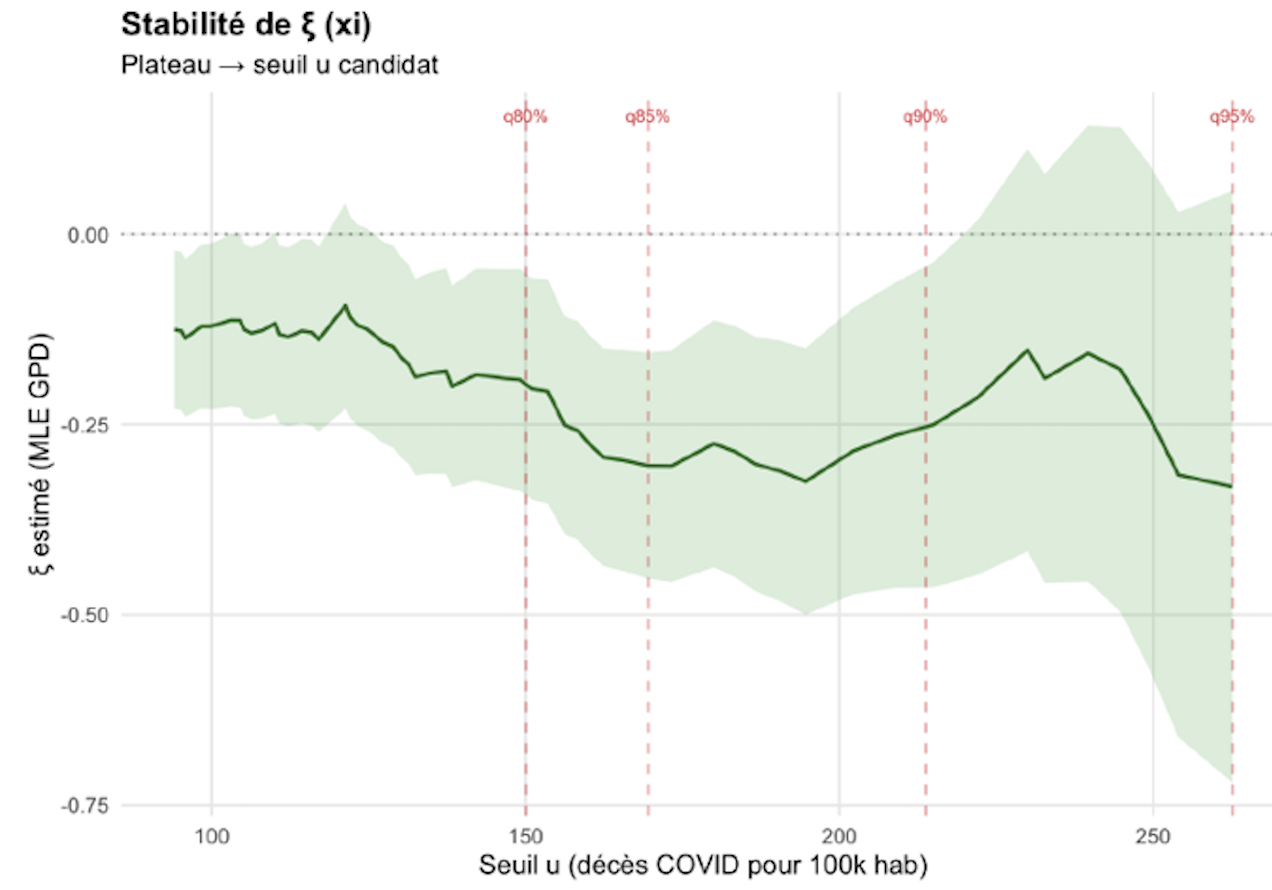
\includegraphics[width=0.7\textwidth]{stabilite.png}
    \caption{Stabilité asymptotique de $\xi$}
\end{figure}

\subsection{L'Arbre EVT-CART (Generalized Pareto Regression Trees)}
L'algorithme EVT-CART partitionne récursivement l'espace pour isoler des sous-populations homogènes. À chaque scission, l'algorithme cherche la variable explicative et le point de coupure qui maximisent la différence de log-vraisemblance de la GPD entre le nœud parent et les nœuds enfants (cf. Annexe).

L'arbre généré (Figure 4) produit 8 feuilles terminales, séparant les comtés notamment par le ratio de personnes âgées, la densité et la géographie spatiale (longitude/latitude).

\begin{figure}[H]
    \centering
    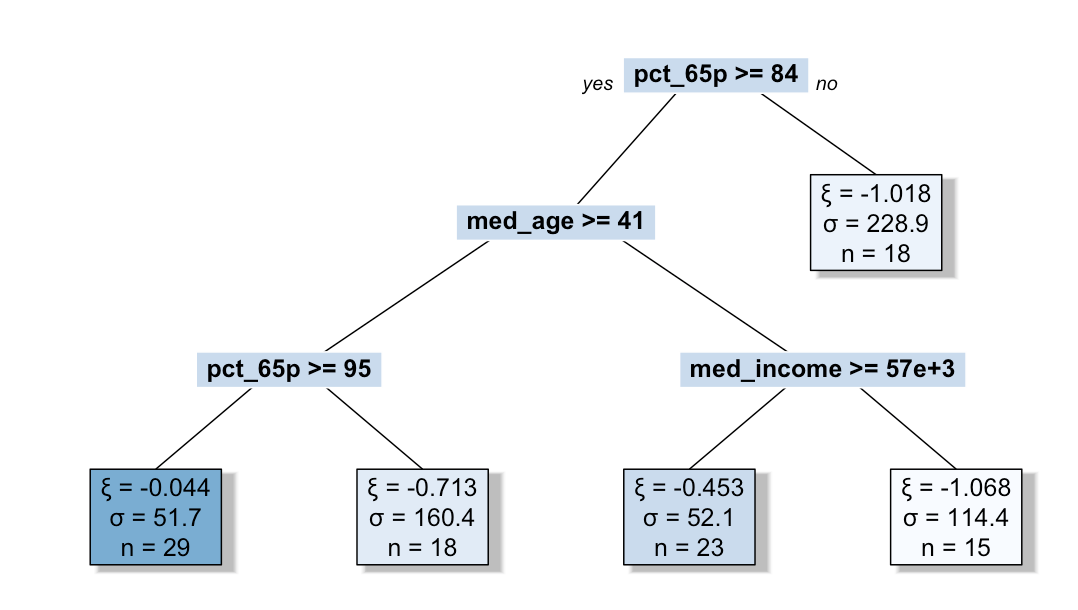
\includegraphics[width=0.7\textwidth]{arbre.png}
    \caption{Arbre EVT-CART ajusté sur les comtés extrêmes.}
\end{figure}

\subsection{Critique des ajustements locaux}
Les diagnostics par feuille prouvent l'efficacité de la segmentation CART :

\begin{itemize}
    \item \textbf{Succès de l'homogénéisation :} Pour 3 feuilles sur 5 (3, 8, 9), l'ajustement empirique (QQ-plots) est excellent. Le paramètre estimé y est \textbf{$\xi < 0$}, signifiant que le modèle a "appris" l'existence d'une borne supérieure physique à la mortalité locale.
    \item \textbf{Écartement en fin de queue (Feuilles 10 et 11) :} L'ajustement y est satisfaisant sur la majorité des points, mais un peu moins précis pour les valeurs les plus extrêmes, où les quantiles empiriques se détachent légèrement de la prédiction théorique. Cette déviation est une limite inhérente à l'EVT en espace réduit : l'arbre a isolé des sous-populations contenant très peu de données, ce qui augmente la variance de l'estimateur du Maximum de Vraisemblance et rend l'extrapolation plus incertaine sur les événements les plus rares.
\end{itemize}

\begin{figure}[H]
    \centering
    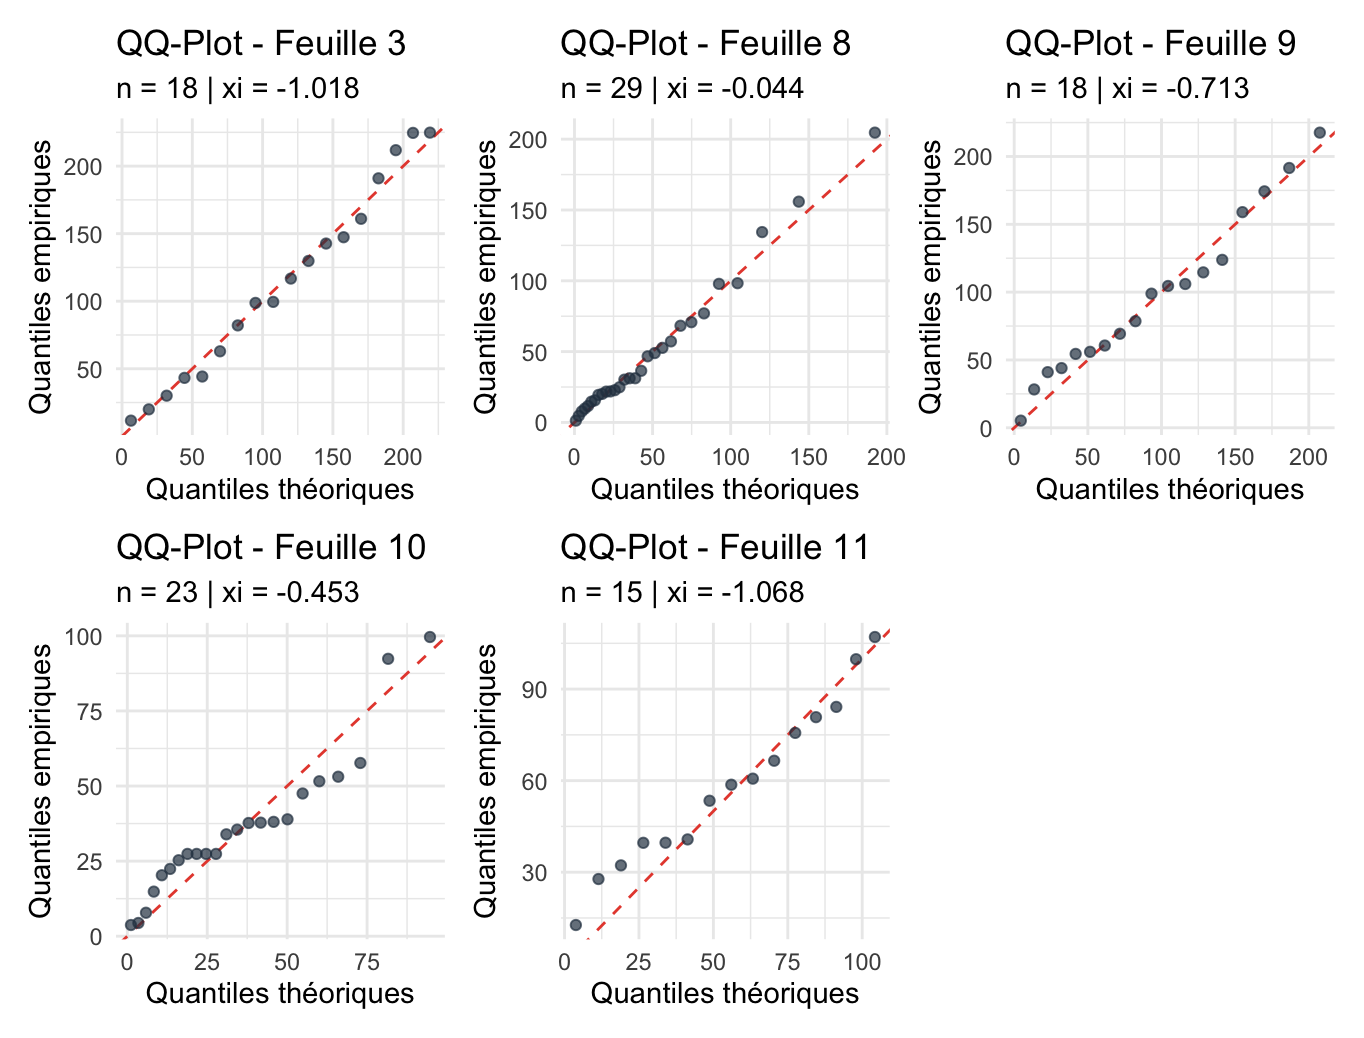
\includegraphics[width=0.9\textwidth]{qq-plots1.png}
    \caption{QQ-plots empiriques vs théoriques démontrant la validité locale (hormis Feuille 5).}
\end{figure}

\begin{figure}[H]
    \centering
    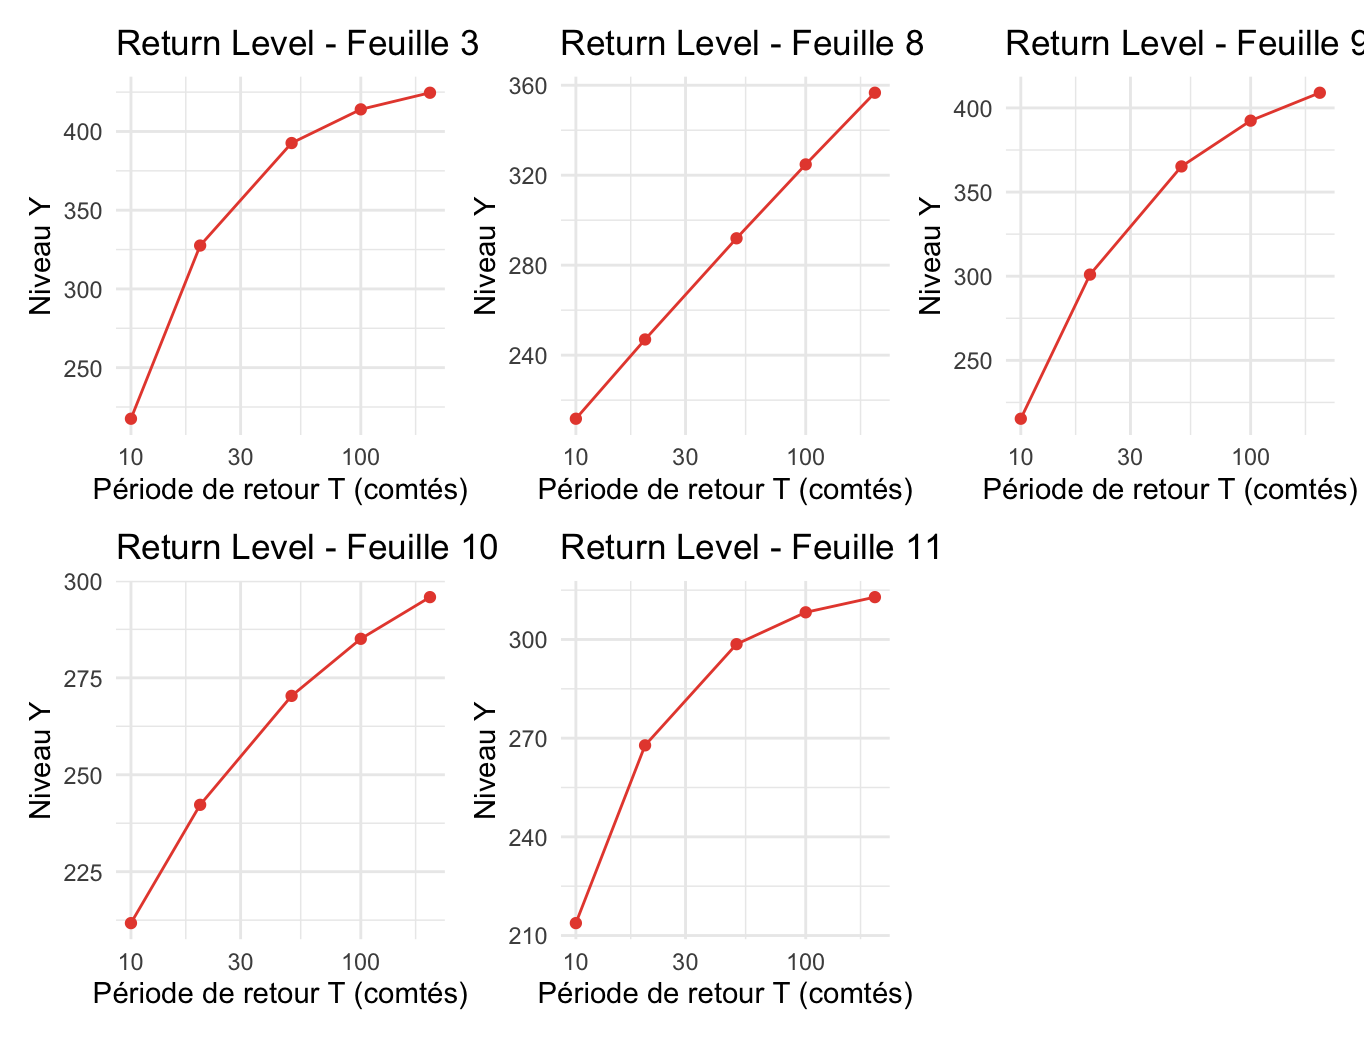
\includegraphics[width=0.9\textwidth]{return1.png}
    \caption{Niveaux de retour (Return Levels) illustrant la forme de la queue de distribution par cluster.}
\end{figure}

\subsection{Améliorations}

\paragraph{Ajout de variables socio-économiques}

Dans un premier temps, nous avons ajouté des variables socio-économiques au jeu de données.

\begin{itemize}
    \item \texttt{pct\_poverty} : taux de pauvreté du comté ;
    \item \texttt{pct\_vaccinated} : couverture vaccinale du comté ;
    \item \texttt{pct\_uninsured} : proportion de personnes sans assurance santé ;
    \item \texttt{rucc} : indice de ruralité du comté.
    \item \texttt{population} : indique la taille de la population
    \item \texttt{total\_deaths} : indice du nombre de morts dans le comté
    \item \texttt{deaths\_male} : indice du nombre d'hommes morts dans le comté
\end{itemize}

L'ajout de ces variables conduit au graphique suivant :

\begin{figure}[H]
    \centering
    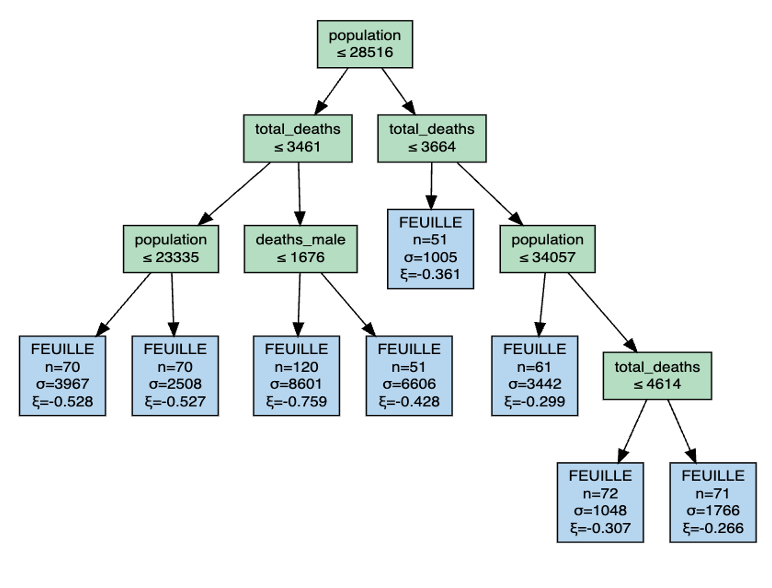
\includegraphics[width=0.8\textwidth]{photo_4}
    \caption{Ajout des variables socio-économiques au modèle EVT-CART.}
\end{figure}

 Le modèle de référence dispose de 7 variables candidates : \texttt{med\_age}, \texttt{med\_income}, \texttt{density}, \texttt{pct\_male}, \texttt{pct\_65p}, \texttt{lon} et \texttt{lat}. Parmi celles-ci, l'algorithme retient pour les splits \texttt{pct\_65p}, \texttt{density}, \texttt{lon}, \texttt{lat} et \texttt{med\_income}, produisant un AIC de 10\,392. Le modèle enrichi ajoute des variables socio-économiques (\texttt{pct\_poverty}, \texttt{pct\_uninsured}, \texttt{pct\_vaccinated}, \texttt{rucc}) ainsi que des variables volumétriques (\texttt{population}, \texttt{total\_deaths}, \texttt{deaths\_male}, \texttt{deaths\_65p}), soit 14 variables candidates au total. Son AIC est meilleur (9\,935), ce qui confirme une segmentation GPD plus homogène.

Le résultat surprenant est le suivant : malgré l'ajout de nombreuses variables socio-économiques pertinentes, l'algorithme choisit de splitter \textbf{exclusivement} sur \texttt{population}, \texttt{total\_deaths} et \texttt{deaths\_male}, ignorant totalement \texttt{pct\_poverty}, \texttt{pct\_uninsured}, \texttt{rucc} ou \texttt{pct\_vaccinated}. Ce comportement est contre-intuitif car on pourrait s'attendre à ce que des variables comme le taux de pauvreté ou le taux de vaccination, reconnues comme déterminants structurels de la mortalité COVID, contribuent à la segmentation. L'explication réside dans la façon dont l'EVT CART split : l'algorithme maximise le gain de log-vraisemblance GPD à chaque n\oe{}ud, et les variables de comptage brut présentent une variance très élevée qui leur permet de créer des groupes beaucoup plus homogènes au sens de la GPD que les proportions socio-économiques. Ces dernières, bien qu'interprétables, produisent des gains marginaux trop faibles pour être sélectionnées en présence des comptages bruts.

\paragraph{Suppression des variables directement corrélées à la cible}

Après observation des résultats du modèle enrichi, nous avons constaté que l'algorithme splittait exclusivement sur les variables de comptage brut (\texttt{total\_deaths}, \texttt{population}, \texttt{deaths\_male}), occultant complètement les variables socio-économiques pourtant pertinentes. Nous avons donc souhaité tester une version du modèle en supprimant ces variables directement liées à la mortalité COVID, afin de voir si des regroupements structurels plus interprétables émergeraient naturellement.

L'objectif est d'éviter que l'arbre ne réalise ses partitions à partir de variables mécaniquement corrélées à la variable cible. En effet, si l'on autorise des variables comme \texttt{total\_deaths} ou \texttt{deaths\_male}, l'arbre peut essentiellement reconstruire la variable cible à partir d'informations déjà très proches d'elle, au lieu d'identifier de véritables facteurs explicatifs structurels. Nous avons donc préféré construire un arbre basé uniquement sur des caractéristiques démographiques, géographiques et socio-économiques, dans l'espoir que des profils territoriaux cohérents — tels que des comtés pauvres, ruraux ou à forte proportion de personnes âgées — émergent comme déterminants naturels des régimes de mortalité extrême.

Les variables finalement retenues sont :

\begin{center}
\begin{itemize}
    \item \texttt{density}
    \item \texttt{area\_km2}
    \item \texttt{med\_income}
    \item \texttt{med\_age}
    \item \texttt{pct\_male}
    \item \texttt{pct\_65p}
    \item \texttt{pct\_uninsured}
    \item \texttt{pct\_vaccinated}
    \item \texttt{rucc}
    \item \texttt{pct\_poverty}
\end{itemize}
\end{center}

L'arbre obtenu est présenté ci-dessous :

\begin{figure}[H]
    \centering
    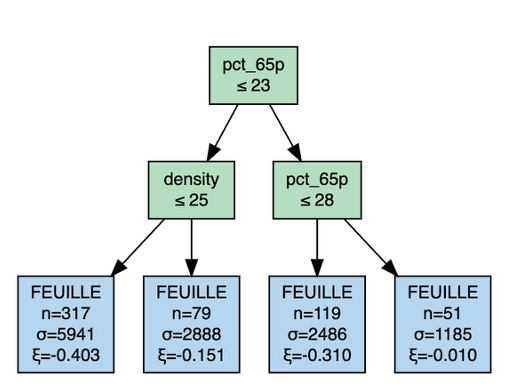
\includegraphics[width=0.7\textwidth]{photo_5}
    \caption{Arbre EVT-CART construit sans variables directement corrélées à la cible.}
\end{figure}


Cette deuxième version, construite uniquement à partir de covariables socio-démographiques et géographiques, produit un arbre à 4 feuilles avec un AIC de 10\,187.8. Toutes les feuilles sont statistiquement distinctes au sens du test de Kolmogorov-Smirnov. Les principaux splits reposent sur les variables \texttt{pct\_65p} et \texttt{density}, deux facteurs connus pour influencer fortement la mortalité COVID.

La première version, intégrant également les variables de mortalité brutes, produit un arbre plus profond à 8 feuilles avec un AIC de 9\,935.8. Cette version est donc meilleure du point de vue du critère AIC.

\paragraph{Analyse de sensibilité des hyperparamètres}

Afin de valider les choix de paramétrage retenus, une analyse de sensibilité a été conduite sur les trois hyperparamètres principaux : le gain minimal de log-vraisemblance (\texttt{min\_gain}), la profondeur maximale (\texttt{max\_depth}) et la taille minimale des feuilles (\texttt{min\_node}), en faisant varier un paramètre à la fois autour des valeurs de référence (\texttt{min\_gain} = 5, \texttt{max\_depth} = 4, \texttt{min\_node} = 50).

Les résultats montrent que l'arbre est stable : diminuer \texttt{min\_gain} en dessous de 5 ne crée aucun split supplémentaire, et augmenter \texttt{max\_depth} au-delà de 4 ne modifie plus la structure de l'arbre. Ces deux observations indiquent que l'algorithme a naturellement épuisé les partitions informatives disponibles. Concernant \texttt{min\_node}, des valeurs plus faibles améliorent légèrement l'AIC mais produisent des feuilles statistiquement non distinctes au test de Kolmogorov-Smirnov, suggérant un sur-découpage. La valeur retenue de 50 garantit des estimations GPD fiables, notamment pour le paramètre de forme $\xi$.

\begin{figure}[H]
    \centering
    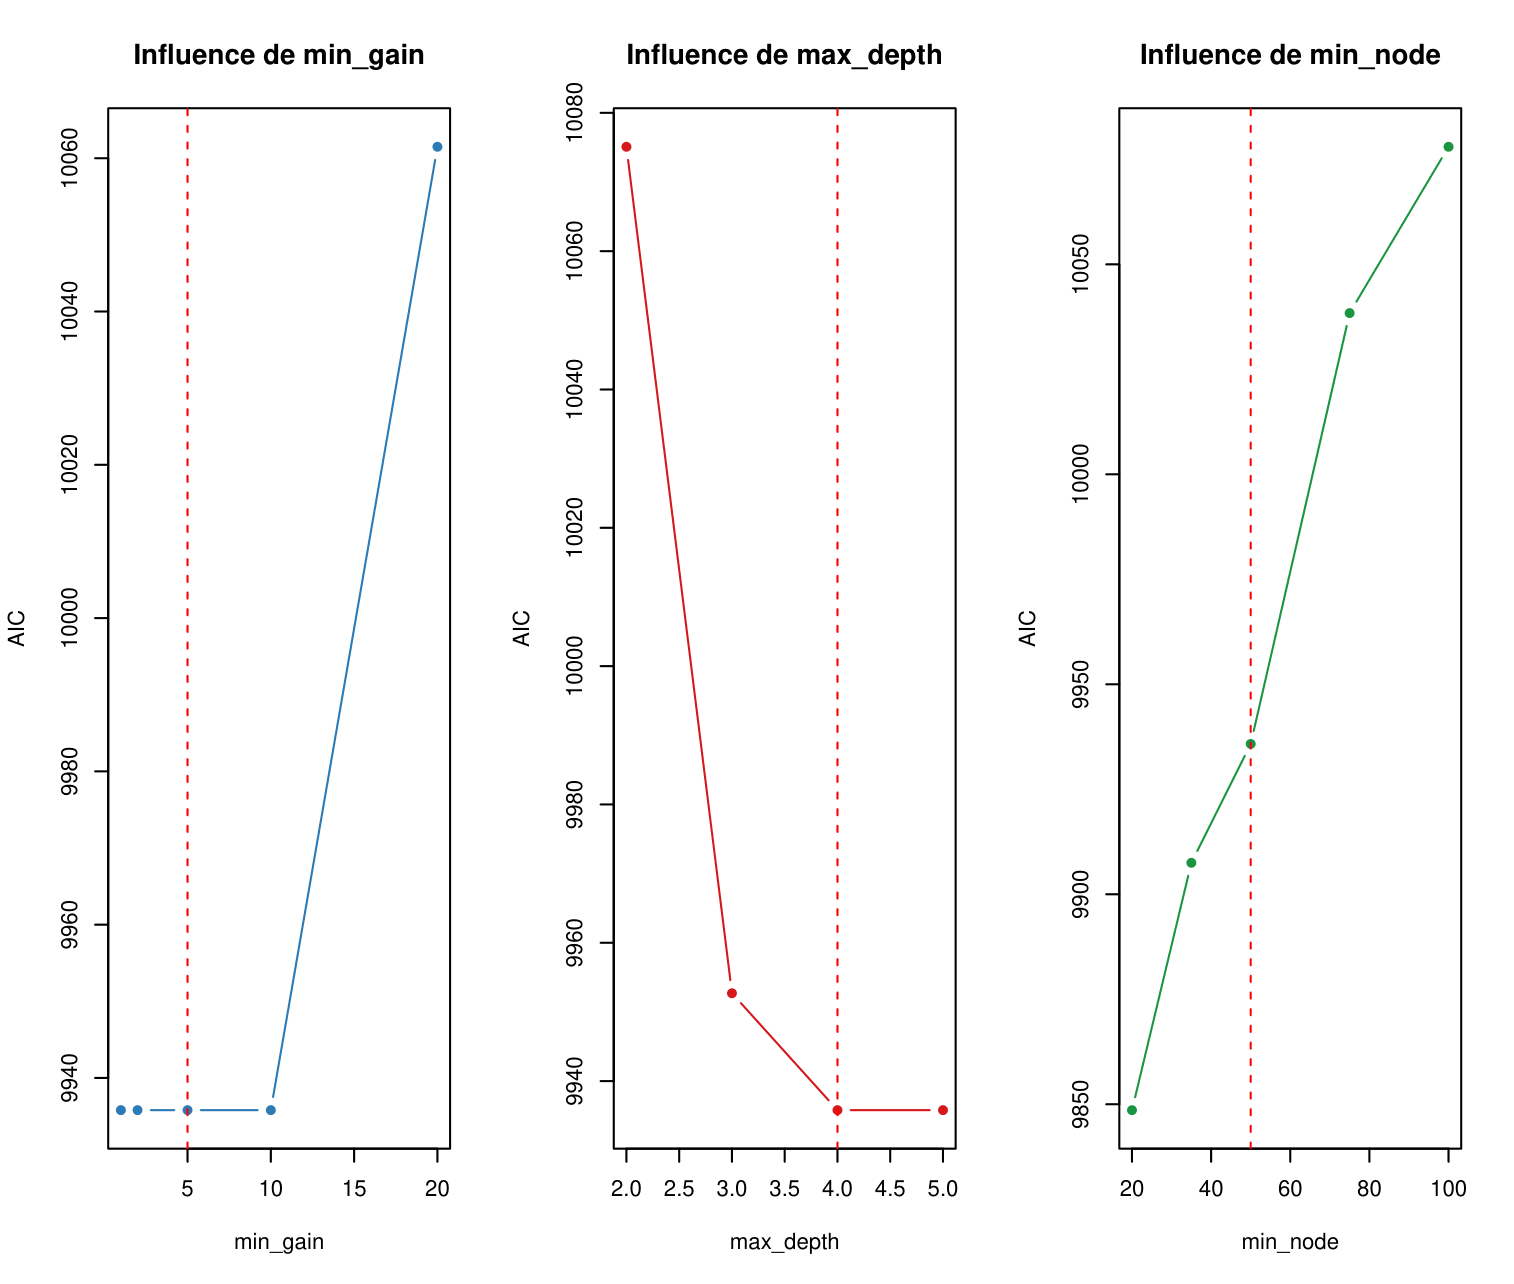
\includegraphics[width=0.8\textwidth, height=6cm]{photo_10.png}
    \caption{Analyse de sensibilité des hyperparamètres de l'arbre EVT-CART.}
\end{figure}

Quelle que soit la configuration testée, l'arbre EVT-CART améliore significativement le modèle GPD global ($AIC = 10\,352$), avec un gain minimal de 174 points d'AIC pour la configuration retenue.
\section{Stratégie de Cartographie Spatiale : Krigeage}

Un enjeu final du projet (répondant aux attentes du "client") était de fournir une cartographie exhaustive et continue du paramètre $\xi$ mesurant le risque extrême. 

Or, d'un point de vue informatique et industriel, le dataset présentait de nombreux "trous" géographiques (comtés sans remontées de données CDC). Pour résoudre ce problème, nous avons adopté une stratégie en deux étapes :
\begin{enumerate}
    \item \textbf{Prédiction via l'arbre :} Tous les comtés présents dans la base ont été passés dans l'arbre pour hériter du paramètre $\xi$ correspondant à leur profil socio-démographique.
    \item \textbf{Krigeage Ordinaire :} Pour les comtés manquants, nous avons modélisé la dépendance spatiale (variogramme) à partir des comtés classifiés, et interpolé les valeurs de $\xi$.
\end{enumerate}

\begin{figure}[H]
    \centering
    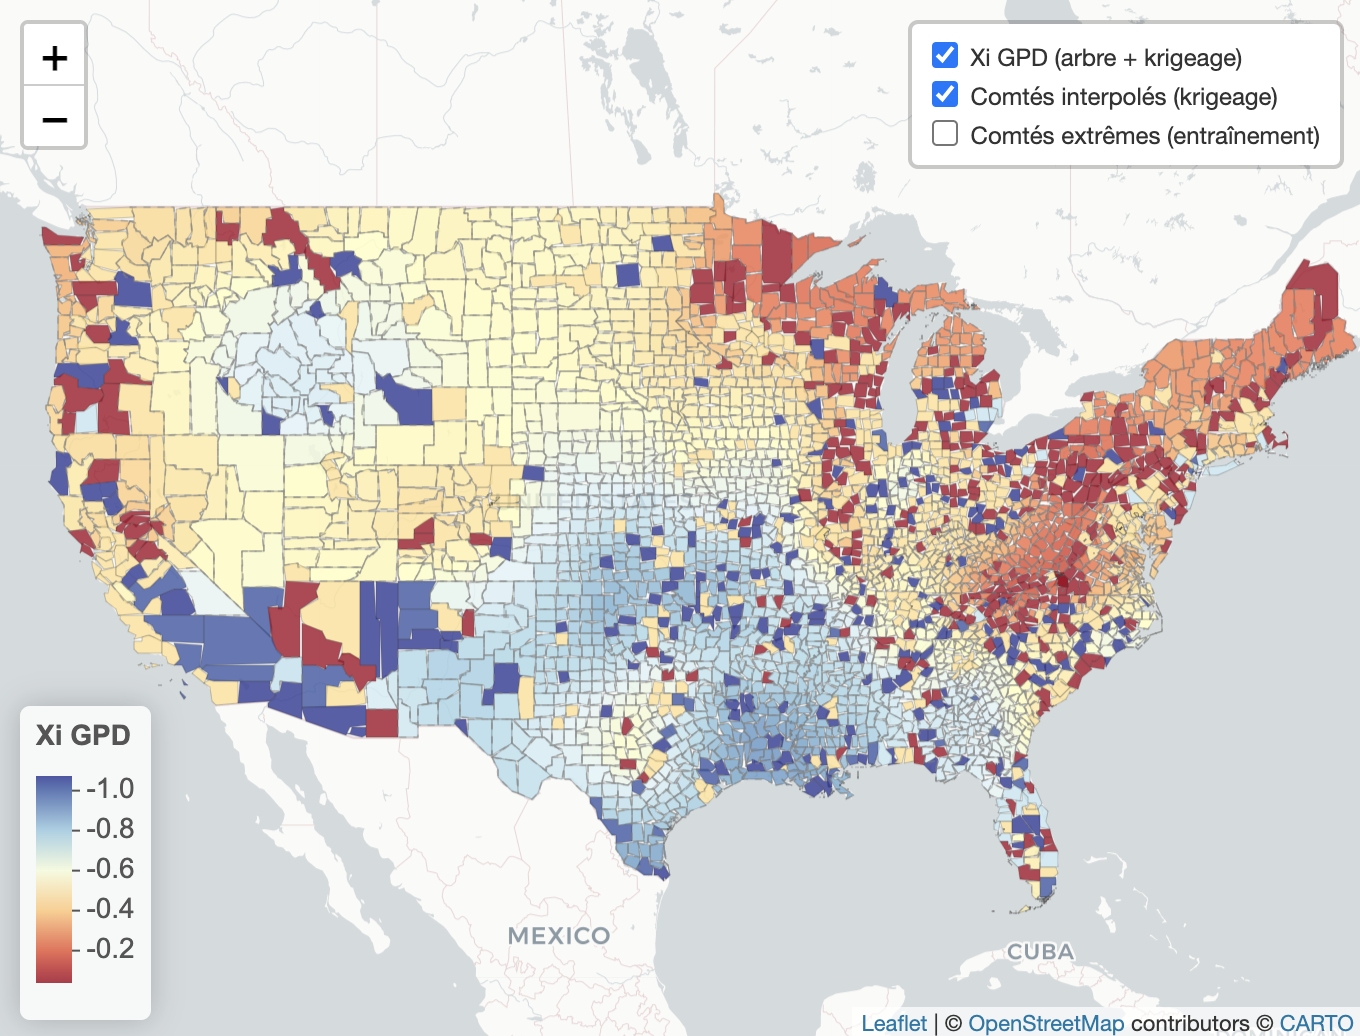
\includegraphics[width=0.9\textwidth]{carte1.png}
    \caption{Carte hybride des risques extrêmes ($\xi$). Les comtés interpolés par krigeage sont hachurés pour différencier la donnée réelle de l'interpolation.}
\end{figure}

\section{Conclusions et Perspectives}

\textbf{Bilan scientifique :} Ce travail démontre formellement l'incapacité d'un modèle global à capter l'hétérogénéité spatiale des pandémies. L'approche EVT-CART a prouvé sa grande pertinence en identifiant des sous-régions partageant la même dynamique (généralement bornée, $\xi < 0$) de scénarios du pire. Le recours géostatistique (Krigeage) a permis de combler les lacunes de données pour proposer une vision territorialisée continue.

\textbf{Valeur ajoutée pour le décideur :} Nous fournissons un outil capable de différencier structurellement un risque maîtrisable (taux plafonné) d'un risque d'emballement systémique (queue lourde). Cela offre une base mathématique robuste pour le dimensionnement et l'allocation préventive de ressources hospitalières ou de fonds assurantiels.

\textbf{Limites et points en suspens :}
Le principal défi méthodologique non résolu réside dans la gestion de la variance sur les petites feuilles terminales de l'arbre (phénomène illustré par la Feuille 5). L'utilisation future d'une estimation bayésienne avec des \textit{priors} géographiques permettrait de régulariser le paramètre $\xi$ et d'éviter ces divergences mathématiques sur les petits échantillons.

Enfin, l'aboutissement applicatif de ce projet sera le déploiement d'une \textbf{application Web RShiny} interactive. Elle intégrera ce pipeline mathématique pour permettre aux utilisateurs finaux d'explorer dynamiquement l'impact du seuil $u$ et des variables explicatives sur la cartographie du risque extrême.

\newpage
\appendix
\section{Annexe : Critère d'optimisation de l'algorithme EVT-CART}

\subsection{Fonction de Log-Vraisemblance Négative}
Dans chaque nœud de l'arbre, l'algorithme estime les paramètres $\theta = (\sigma, \xi)$ qui ajustent au mieux les $n_u$ excès observés $y_i = Y_i - u$. 

\begin{tcolorbox}[colback=white, colframe=bordergray, title=Negative Log-Likelihood (NLL)]
La log-vraisemblance négative à minimiser est donnée par l'expression :
\begin{equation}
    \mathcal{L}(\sigma, \xi \mid y) = n_u \ln(\sigma) + \left(1 + \frac{1}{\xi}\right) \sum_{i=1}^{n_u} \ln\left(1 + \frac{\xi y_i}{\sigma}\right)
\end{equation}
\textit{Sous la contrainte de validité du support : $(1 + \xi y_i / \sigma) > 0$.}
\end{tcolorbox}

\subsection{Critère de Scission (Déviance)}
Le principe fondamental de CART est de minimiser l'hétérogénéité intra-classe. Dans le cadre de l'EVT-CART développé par Farkas et al. (2021), l'impureté d'un nœud est évaluée par sa Déviance $D$, définie comme le double de sa NLL minimale.

Pour une scission candidate $s$ séparant un nœud parent en deux enfants (Gauche $L$ et Droit $R$), le gain d'information est :
\begin{equation}
    \Delta D(s) = D_{parent} - (D_L + D_R)
\end{equation}
L'arbre procède de manière gloutonne (\textit{greedy approach}) en sélectionnant itérativement la variable et le point de coupure qui maximisent ce gain $\Delta D(s)$.

\newpage


\newpage

\begin{thebibliography}{9}
\bibitem{coles} 
Coles, S. (2001). 
\textit{An Introduction to Statistical Modeling of Extreme Values}. Springer Series in Statistics.
\bibitem{thomas}
Thomas, M. (2022).
\textit{Contributions à la théorie des valeurs extrêmes et à la gestion du risque}. Support de webinaire, Sorbonne Université.
\bibitem{farkas} 
Farkas, J., Heranval, A., Lopez, O., \& Thomas, M. (2021). 
\textit{Generalized Pareto Regression Trees for extreme events analysis}. arXiv preprint arXiv:2112.10409.
\end{thebibliography}

\end{document}
